\documentclass[12pt]{article}

\usepackage{graphics}
\usepackage{graphicx}
\usepackage{hyperref}
\hypersetup{
    colorlinks=true, %set true if you want colored links
    linktoc=all,     %set to all if you want both sections and subsections linked
    linkcolor=black,  %choose some color if you want links to stand out
}

\begin{document}

\tableofcontents

\section{What is Parser?}

Parser is that phase of compiler which takes token string as input and with the help of existing grammar, converts it into the corresponding parse tree. Parser is also known as Syntax Analyzer.

\section{Types of Parser}

Parser is mainly classified into 2 categories: 

\begin{itemize}
	\item Top-down Parser
	\item Bottom-up Parser
\end{itemize}

\begin{center}
	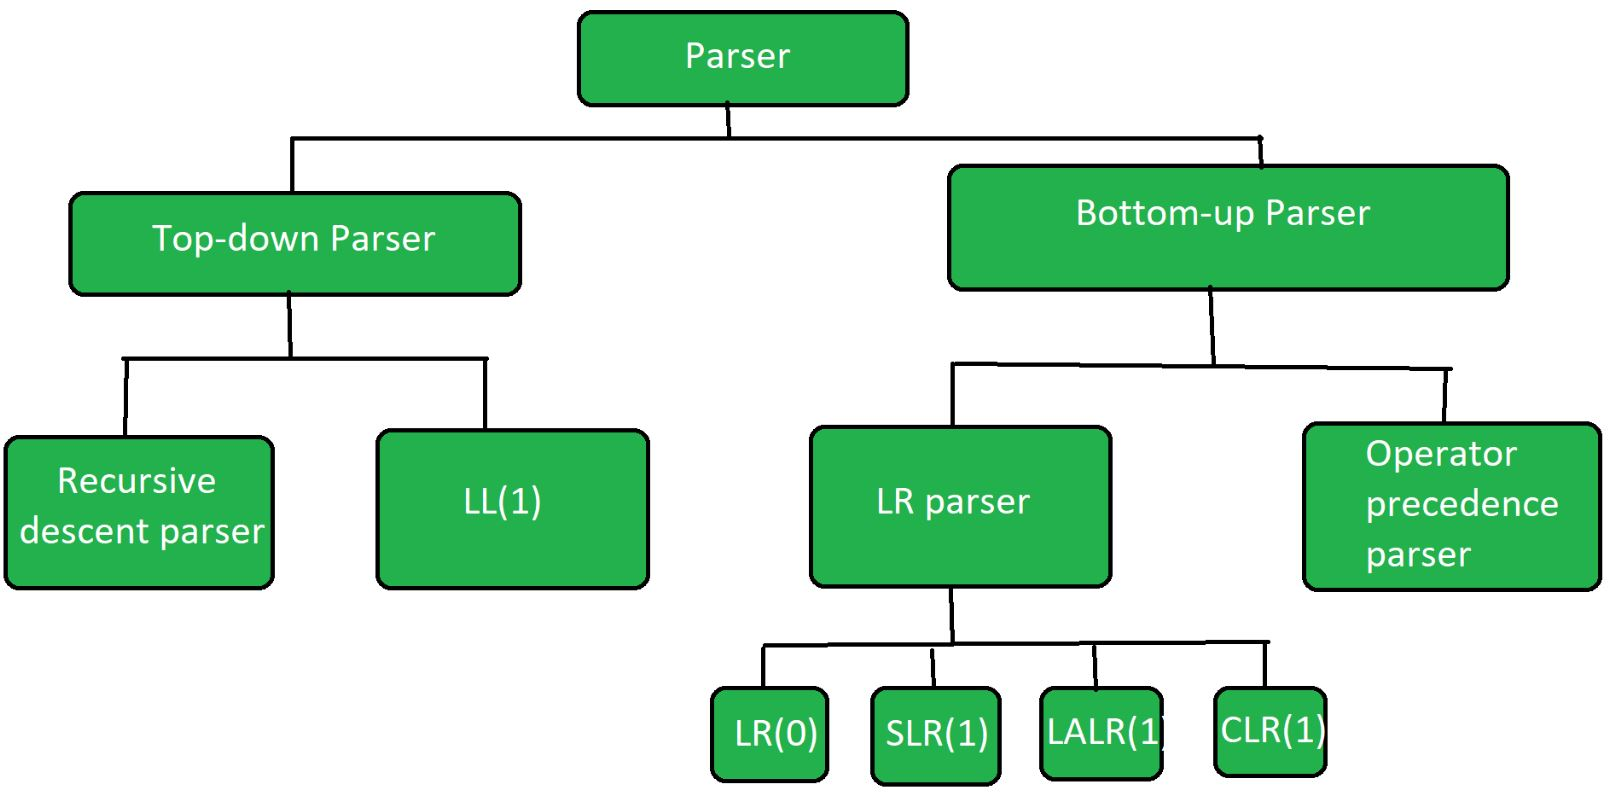
\includegraphics[scale=.4]{./parser.jpg}
	%\caption{}
\end{center}


These are explained as below.


\section{Top-down Parser}

Top-down parser is the parser which generates parse for the given input string with the help of grammar productions by expanding the non-terminals i.e. it starts from the start symbol and ends on the terminals. It uses left most derivation. Further Top-down parser is classified into 2 types: Recursive descent parser, and Non-recursive descent parser.

\begin{itemize}
	\item \textbf{Recursive descent parser :} It is also known as Brute force parser or the with backtracking parser. It basically generates the parse tree by using brute force and backtracking.
	\item \textbf{Non-recursive descent parser :} It is also known as LL(1) parser or predictive parser or without backtracking parser or dynamic parser. It uses parsing table to generate the parse tree instead of backtracking.
\end{itemize}



\section{Bottom-up Parser}

Bottom-up Parser is the parser which generates the parse tree for the given input string with the help of grammar productions by compressing the non-terminals i.e. it starts from non-terminals and ends on the stat symbol. It uses reverse of the right most derivation.
Further Bottom-up parser is classified into 2 types: LR parser, and Operator precedence parser.

\begin{itemize}
	\item \textbf{LR parser : }
	
	LR parser is the bottom-up parser which generates the parse tree for the given string by using unambiguous grammar. It follow reverse of right most derivation.
LR parser is of 4 types: 
	\begin{itemize}
		\item LR(0)
		\item SLR(1)
		\item LALR(1)
		\item CLR(1) 
	\end{itemize}
	\item \textbf{Operator precedence parser : }
	
	It generates the parse tree form given grammar and string but the only condition is two consecutive non-terminals and epsilon never appear in the right-hand side of any production.
\end{itemize}




\end{document}